In this test problem, an initially flat fluid surface is perturbed, and waves
from this perturbation travel to the boundary and reflect back into the
domain. This problem might, for example, simulate a droplet of water in
a bathtub.
Figure \ref{fig:bathtub_initial} shows this initial perturbation on the fluid
surface, representing the droplet of water falling into the bathtub.

%-------------------------------------------------------------------------------
\begin{figure}[ht]
   \centering
   \begin{subfigure}{0.45\textwidth}
      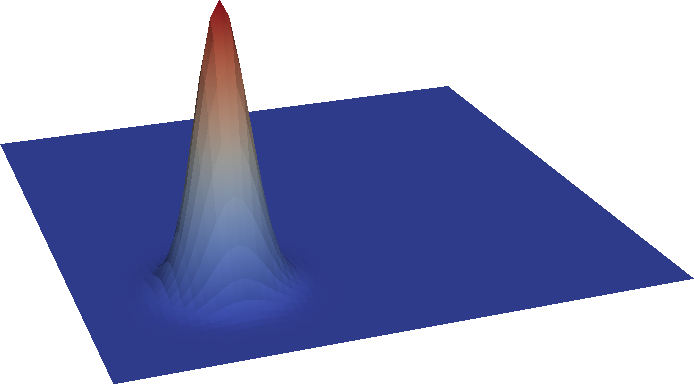
\includegraphics[width=\textwidth]
        {\contentdir/results/shallowwater/bathtub/images/initial_shape.png}
      \caption{Surface plot of $\height_0$}
   \end{subfigure}
   \begin{subfigure}{0.45\textwidth}
      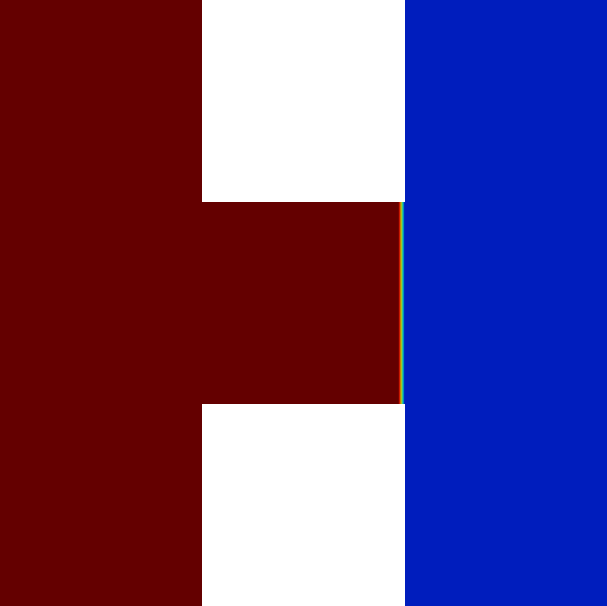
\includegraphics[width=\textwidth]
        {\contentdir/results/shallowwater/bathtub/images/initial.png}
      \caption{Color map of $\height_0$}
   \end{subfigure}
   \caption{Initial Height Profile for the Bathtub Test Problem}
   \label{fig:bathtub_initial}
\end{figure}
%-------------------------------------------------------------------------------

The problem parameters are summarized in Table \ref{tab:bathtub}.
The simulations were performed on a $64\times 64$-cell mesh, with
a constant time step size of $\dt = 0.002$, run until $t = 0.5$.
For the entropy viscosity method, the entropy residual coefficient
and entropy jump coefficient were set to $\entropyresidualcoef=1$
and $\entropyjumpcoef=1$, respectively.

%-------------------------------------------------------------------------------
\begin{table}[htb]\caption{Bathtub Test Problem Summary}
\label{tab:bathtub}
\centering
\begin{tabular}{l l}\toprule
\emph{Parameter} & \emph{Value}\\\midrule
Domain & $\mathcal{D} = (0,1)^2$\\
Initial Conditions & $\height_0(\x)=1 + e^{-250((x-0.25)^2+(y-0.25)^2)}$\\
                   & $\velocity_0(\x) = \mathbf{0}$\\
Boundary Conditions & $\nabla\height(\x,t)=0
  \eqc \quad \x\in\partial\mathcal{D}\eqc \quad t>0$,\\
                    & $\velocity\xt\cdot\normalvector = 0
  \eqc \quad \x\in\partial\mathcal{D}\eqc \quad t>0$,\\
Bathymetry & $\bathymetry(\x)=0$\\
\bottomrule\end{tabular}
\end{table}
%-------------------------------------------------------------------------------

Figure \ref{fig:bathtub} shows a comparison of the solutions of the low-order
invariant domain method vs. the entropy viscosity method. Solutions were obtained
using explicit Euler time discretization and are compared at $t = 0.1$ and
$t = 0.5$.

The entropy viscosity solution is shown here to be much sharper than
the low-order method. It is already
clear at $t = 1$ how much diffusion the low-order scheme introduces; by
$t = 5$, wave forms are hardly visible, as opposed to the results shown
by the entropy viscosity method, where the reflected wave forms are
clearly visible: four waves can be identified in Figure \ref{fig:bathtub_EV_t05}:
\begin{enumerate}
  \item the main, largest wave, going from roughly (0,0.75) to (0.75,0),
  \item a wave going from roughly (0,0.25) to (0.75,0),
  \item a wave going from roughly (0,0.75) to (0.25,0), and
  \item the smallest wave, going from roughly (0,0.25) to (0.25,0).
\end{enumerate}
If one reflects wave 2 about $y=0$, wave 3 about $x=0$, and wave 4 about
both $y=0$ and $x=0$, then one constructs the circular wave form
that would have formed from the droplet in an infinite domain.
The Galerkin method was also applied to this problem, but
when the initial circular wave from the droplet crashed into the boundary,
severe oscillations developed and grew. This was also the case using
SSPRK33, although the oscillations grew more slowly.

As of yet, no FCT method for the 2-D shallow water equations has
been developed in this research because the characteristic transformation performed by the
limiter described in this dissertation cannot simultaneously be applied in
both $x$ and $y$ directions. In this case, the entropy viscosity method
does not encounter noticeable oscillations, but more challenging test
problems, such as a 2-D dam break, could reveal oscillations.

%-------------------------------------------------------------------------------
\begin{figure}[ht]
   \centering
   \begin{subfigure}{0.45\textwidth}
      
\includegraphics[width=\textwidth]
        {\contentdir/results/shallowwater/bathtub/images/low_t01.png}
      \caption{Low-Order, $t=0.1$}
   \end{subfigure}
   \begin{subfigure}{0.45\textwidth}
      
\includegraphics[width=\textwidth]
        {\contentdir/results/shallowwater/bathtub/images/low_t05.png}
      \caption{Low-Order, $t=0.5$}
   \end{subfigure}
   \begin{subfigure}{0.45\textwidth}
      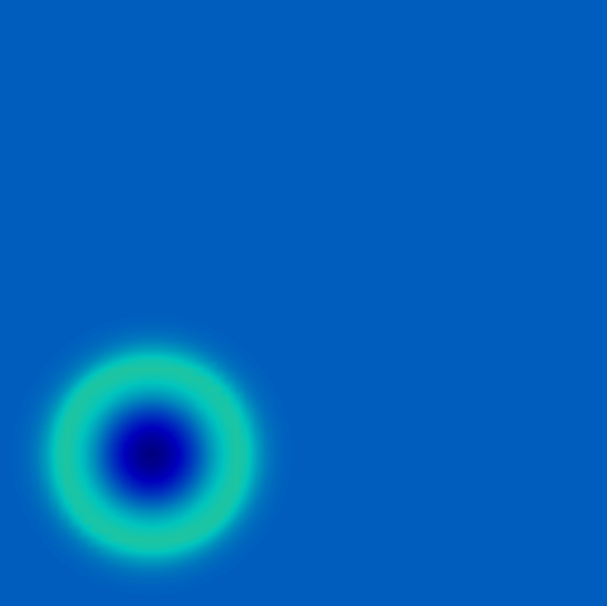
\includegraphics[width=\textwidth]
        {\contentdir/results/shallowwater/bathtub/images/EV_t01.png}
      \caption{EV, $t=0.1$}
   \end{subfigure}
   \begin{subfigure}{0.45\textwidth}
      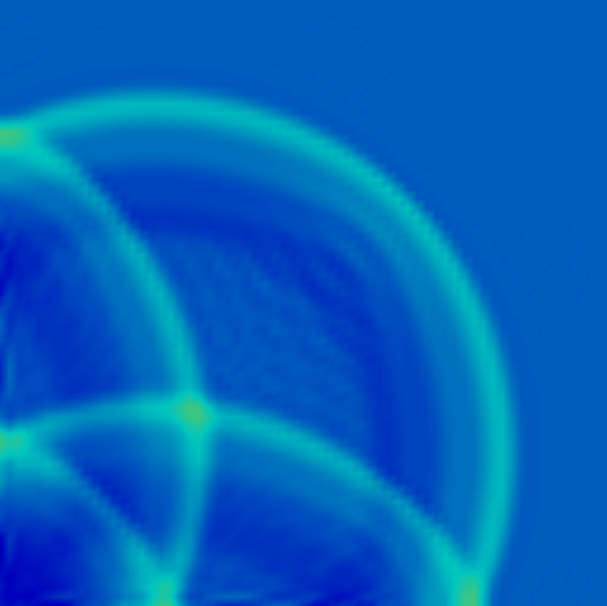
\includegraphics[width=\textwidth]
        {\contentdir/results/shallowwater/bathtub/images/EV_t05.png}
      \caption{EV, $t=0.5$\label{fig:bathtub_EV_t05}}
   \end{subfigure}
   \caption{Comparison of Low-Order and High-Order Solutions for the
     Bathtub Test Problem Using Explicit Euler Time Discretization}
   \label{fig:bathtub}
\end{figure}
%-------------------------------------------------------------------------------

\clearpage
